\chapter{Solution}
\section{Introduction}
Dans le chapitre précédent, nous avons présenté les différentes dimensions du problème de gestion de ressource dans les environnements fog, et nous avons vu également l’importance de cette dernière pour la concrétisation de cedit paradigme.
Nous définirons dans ce chapitre notre solution de conception en nous basant sur les différents travaux traitant du sujet.
\section{Motivation}
Une bonne gestion de ressource permet d'accroître les performances globales du système, en réduisant le temps d'exécution des différentes applications, la latence, ainsi que les coûts énergétiques. Elle permet aussi d’exploiter au mieux les ressources matérielles disponibles, ce qui augmente le rendement et la rentabilité économique des différents équipements.\\ 
Par conséquent, le développement d’un bon modèle de gestion de ressource se révèle d’une importance capitale pour une exploitation efficace et rentable d’une infrastructure fog.
\section{Problématique}
Suite à l’étude des travaux qui traitent de l’amélioration et de l’optimisation de la gestion des ressources, on constate que le problème de planification des ressources est un problème central qui nécessite d'être investigué afin d’effectuer une gestion de ressource optimale. \\
Le problème consiste à concevoir un modèle de planification de ressource dynamique,efficace et évolutif, qui permet affecter les différentes demandes de ressources, effectuées par les appareils iot, au différent nœud fog d’une manière à optimiser au mieux certaines métriques de liées aux coûts.
\section{État de l’art}
Pour la réalisation de ce travail, on s’est inspiré d’un article publié  traitant partiellement du sujet. \\
Dans ce travail, les auteurs s’intéressent au processus d'approvisionnement dans un environnement cloud, dans lequel ce dernier peut être principalement décomposé en 3 étapes majeures que sont : 
\begin{enumerate}
    \item L’identification des noeuds concernés (c.-à-d. les nœuds sous-utilisés ou sur-utilisés). 
    \item Sélection des VM à migrer.
    \item Réallocation des VM aux nœuds sous-utilisés.
\end{enumerate}
La partie qui nous intéresse étant la troisième étape,  où ils ont proposé un mécanisme d’affectation de VM aux nœuds adéquat, modélisé comme étant un problème de correspondance (matching problem).
\section{Conception de la solution}
\subsection{Hypothèses}
La solution proposée nécessite de faire des hypothèses sur la topologie physique de l’infrastructure fog qui l’implémente.\\
On suppose que : 
\begin{itemize}
    \item La topologie est statique durant l’exploitation, c-a-d qu' une fois la solution implémentée, la topologie ne subit pas de modification.
    \item La topologie suit une organisation matricielle, c-a-d que les nœuds fog sont organisés en des niveaux bien distincts avec le même nombre de nœuds dans chaque niveau.
    \item La topologie est maillé entre les niveaux, c-a-d chaque nœud fog du cluster est relié physiquement à tous les nœuds du niveaux supérieure.
    \item Chaque noeud à une connaissance de tous ses noeud parent et ses noeuds enfants (c-a-d respectivement les noeud du niveaux supérieur et les noeud du niveaux inférieur)
    \item Dans ce modèle, on dispose au minimum de trois type de requête que sont : \\
          \begin{itemize}
             \item La requête demande, qui correspond à une demande de services émise par les appareils IoT, elle comporte tous les détails de la demande.
             \item la requête résultat, qui est généré après l’exécution d’une demande de service, elle est émise à destination de l'appareil émetteur.
             \item La requête jeton, qui représente le jeton circulant entre les différents nœuds passerelle.
          \end{itemize}
\end{itemize}
\subsection{Topologie}
Comme vu précédemment, une infrastructure fog est décomposé de 3 couches superposés que sont :
\begin{itemize}
    \item \emph{La couche IoT}, qui représente l’ensemble des appareils iot qui effectue des demande de service.
    \item \emph{La couche Fog}, qui représente l’ensemble des nœuds fog se trouvant à l’intermédiaire entre les appareils IoT et le cloud.
    \item \emph{La couche cloud} qui représente l’infrastructure cloud traditionnelle.
\end{itemize}
\begin{figure}[H]
    \centering
    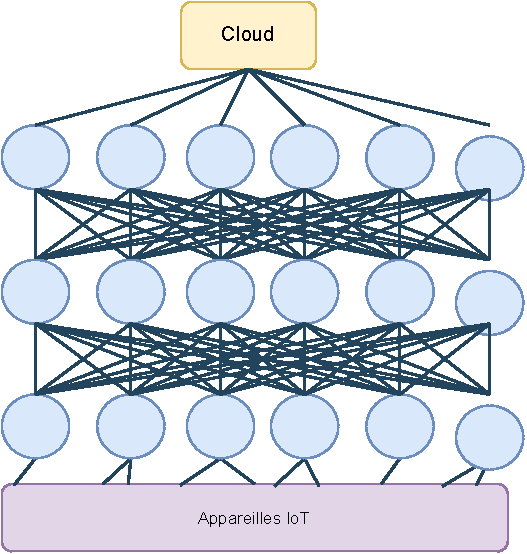
\includegraphics[]{Topologie_générale de_l'infrastructure.pdf}
    \caption{Schémas représentant une architecture fog traditionnelle}
    \label{fig:Topologie_generale de_linfrastructure}
\end{figure}
La solution proposée commence par découper la couche fog de l'infrastructure en un ensemble cluster, c-a-d chaque cluster regroupe un ensemble de nœud fog. Ensuite, chaque cluster est découpé en 2 couche superposé, que sont :
\begin{itemize}
    \item \emph{La couche des nœuds passerelles :} : cette couche est composé du niveau connecté directement à la couche iot.
    \item \emph{La couche des nœuds Fog restant :} qui est composée des niveaux restants.
\end{itemize}
\begin{figure}[H]
    \centering
    \includegraphics[]{ShémaCluster.pdf}
    \caption{Schémas représentant une architecture fog répartie en cluster}
    \label{fig:Infrastructure_fog_repartie_en_cluster}
\end{figure}
\subsection{Scénario}
Ce scénario s’applique pour un cluster, il suffira par la suite de généraliser ce fonctionnement à l'ensemble des cluster défini par l’infrastructure.\\
Les nœuds passerelle du cluster, c-a-d les nœuds connectés directement à la couche iot, reçoivent des demandes de services des différents appareils iot. Chaque nœud préserve ses demandes dans une file en attendant leur correspondance puis leur envoi à leur destination.\\
On définit un jeton circulant d’un nœud passerelle à un autre suivant la politique du tourniquet (round robin). Si un nœud passerelle possède le jeton alors il effectue une correspondance des demandes qui se trouve dans sa file avec les nœuds fog du cluster, puis il envoie chaque demande au nœud fog correspondant, et  renvoie le jeton au prochain nœud passerelle et ainsi de suite.
\begin{figure}[H]
    \centering
    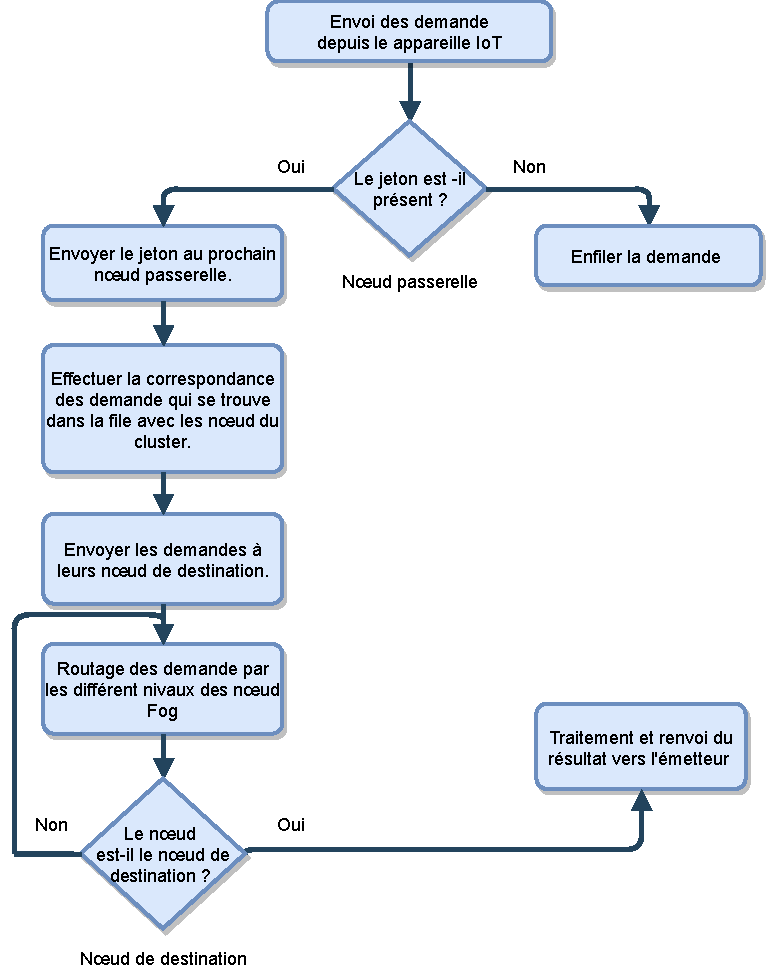
\includegraphics[]{Organigramme-scenario globale.pdf}
    \caption{Organigramme qui illustre les scénarios depuis la réception de la demande jusqu’au retour du résultat du traitement}
    \label{fig:Topologie_generale de_linfrastructure}
\end{figure}
\subsection{Description algorithmique du scénario}
La solution est conçue suivant le paradigme événementiel, c-a-d une approche de l’algorithmique basé sur la notion d'événement, ou on cherche à associer à chaque événement une procédure à exécuter appelée “Routine”.   
Notre solution comporte 2 routine principales que sont :
\begin{itemize}
    \item \emph{La routine associé au noeud passerelle}
    \item \emph{La Routine associé au noeud Fog}
\end{itemize}
\subsubsection{Routine associée au nœud passerelle}
Cette routine est exécutée au niveau des nœuds passerelle à chaque fois qu’une requête est reçue.
Le pseudo code de cette routine est le suivant :\\
\begin{algorithm}[H]
 %\KwData{this text}
 %\KwResult{how to write algorithm with \LaTeX2e }
 \eIf{Requête reçus est de type jeton}
 {  
    // Appeler la  procédure Correspondance.\\
    Correspondance (fileDemande, listeNoeuds);\\
    // Puis on effectue le routage des demandes.\\
   \ForEach{Demande $D_i \in fileDemande$}
   {
     \eIf{listeParents.contient($D_i$.destination)}
     {envoyer(demande, $D_i$.destination);}
     {
         envoyer(demande, NoeudPèreParDéfaut);\\
        // on met à jour le nœud par défaut à chaque fois afin d'équilibrer la charge entre les différentes liaisons.\\
	    NoeudPèreParDéfaut \gets prochainNoeudParent();\\
     }
   }
 }
 {
   \eIf{Requête reçus est de type résultat}
   {// envoyer le résultat à l'appareil iot concerné.\\
       \eIf{resultat.destinatinon est relié à ce noeud}
       {envoyer(resultat,resultat.destination);}
   }
   {// la requête est par conséquent de type demande.\\
     Enfiler( fileDemande,Demande);
   }
 }
 \caption{Routine associée aux nœuds passerelles\\ \\}
\end{algorithm}
 \paragraph{Procédure de correspondance :}\\
 Pour l’implémentation de cette procédure, nous avons opté pour l’utilisation de l’algorithme de gale-shapley, qui est un algorithme conçu pour résoudre le problème des mariages stables.\\
Il présente des propriété intéressante que sont :
\begin{itemize}
    \item De bonne performance dû à sa complexité quadratique.
    \item A sa terminaison toute demande sera associée à un nœud.
    \item Les couples (demande,nœud) résultant de cet algorithme sont stables.
    \item La configuration résultante est optimale en comparaison à toutes les autres solutions stables.
\end{itemize}
Cet algorithme nécessite la définition d’une relation de préférence, qu’on nommera dans cette solution “Relation d’adéquation” qui est associée à chaque demande et à chaque nœud. \\
Pour ce faire, on définie une distance entre la demande et le noeud qui calculer de la manière suivante :
\begin{center}
    $$Distance =\left \lbrace 
    \begin{array}{ll}
        \frac{C_u + Cdem}{C_fd}/ & \mbox{si $C_r > C_{dem}$}\\
        -1 & \mbox{sinon}
    \end{array}
\right.$$
\end{center}
La relation de d’adéquation est définie par la distance minimale entre le nœud et la demande.\\
Autrement dit, soit $D=\{D_1,D_2,..,D_n\}$ un ensemble de demande, et soit $N=\{N_1,N_2,..,N_n\}$.\\
On dit que le noeud $N_i$ est le mieux adéquat à la demande $D_j$ ssi \\
$Distance(D_j,N_j) = Min (Distance(D_j,N_m)), \forall m \in \{1,..,n\}$.\\
\newpage
\textbf{Pseudo code de la procédure :}\\
\begin{algorithm}[H]
\KwData{ListeDemandes, ListeNoeuds}
// initialisation de toute les demandes à une destination null\\
\ForEach{Demande $D_i \in ListeDemandes$}
{
 // on affecte le noeud à la demande.\\
 $D_i$.destination \gets null;\\
}
\While{$\exists$ une\ demande\ $d$\ non\ affecté\ qui\ peut\ se\ proposer\ à\ un\ noeud}
{
n \gets le\ noeud\ le\ mieux\ adéquat\ à\ $d$\ parmi\ la\ liste\ des\ demandes;\\
\eIf{$n$ est libre}
{
  d.destination \gets n;\\
}
{
// si le noeud n’est pas libre et que $d$ est plus adéquate que la demande associé à n.\\
 \eIf{distance(n,n.demande) >distance(n,d)}
 {
   // la demande associé à n est remplacer par d.\\
   n.demande \gets d;\\
 }
}
}
 \caption{Procédure de correspondance\\ \\}
\end{algorithm}
\subsubsection{Routine associé au noeud fog :}
Cette routine est exécutée au niveau des nœuds passerelle à chaque fois qu’une requête est reçue.\\
\textbf{Pseudo code de la routine :}\\
\begin{algorithm}[H]
 %\KwData{this text}
 %\KwResult{how to write algorithm with \LaTeX2e }
 \eIf{Requête reçus est de type demande}
 {  
    \eIf{demande.destination correspond au noeud lui même}
    { executer(demande);\\
     // puis effectuer le routage du résultat.\\
     \eIf{listeEnfants.contient(resultat.destination)}
     {envoyer(resultat, resultat.destination);\\}
     {envoyer(resultat, NoeudFilsParDefaut);\\}
     }
    {  // le noeud en question n’est pas la destination.\\
     \eIf{listeParents.contient(demande.destination)}
     {envoyer(demande, demande.destination);\\}
     {envoyer(demande,NoeudPèreParDéfaut);\\}
   }
 }
 { // la requête reçue est par conséquent une requête résultat.\\
   \eIf{listeEnfants.contient(resultat.destination)}
   {envoyer(resultat, resultat.destination);\\}
   {envoyer(resultat, NoeudFilsParDefaut);\\
   NoeudFilsParDéfaut \gets prochain noeud Fils ;}
 }
 \caption{Routine associée aux nœuds passerelles\\ \\}
\end{algorithm}
